\section{Discussion}
We presented an efficient solution for solving common practical multi-marginal optimal transport problems.
Our construction is significantly cheaper to compute compared to similar methods,
and allows for large numbers of distributions to be matched in common DNN pipelines. 
Our implementation allows imposing fairness constraints for a variety of applications, including those with many groups, without the need for pairwise measures.
As such, subgroup fairness \citep{kearns2018preventing} is an interesting problem setting that we believe can benefit.
% generalized Earth Mover's objective in the context of a setting where we are interested in bringing a set of distributions closer together. 
% Our construction provides significant computational gains over barycentric approaches for estimating higher dimensional distances. Taking advantage of a direct linear programming formulation, we identify readily available gradients that allow for simple incorporation of the generalized EM measure in existing optimization pipelines. We present empirical evidence that our formulation is faster and valuable in some applications.
%Future work may include exploring the practical application and value of the key theoretical result from \cite{kline2019properties} regarding 
Other properties such as 
Minkowski additivity that have not been 
explicitly leveraged in our experiments may also be a worthwhile direction to explore.
\begin{figure}
    \centering
    % 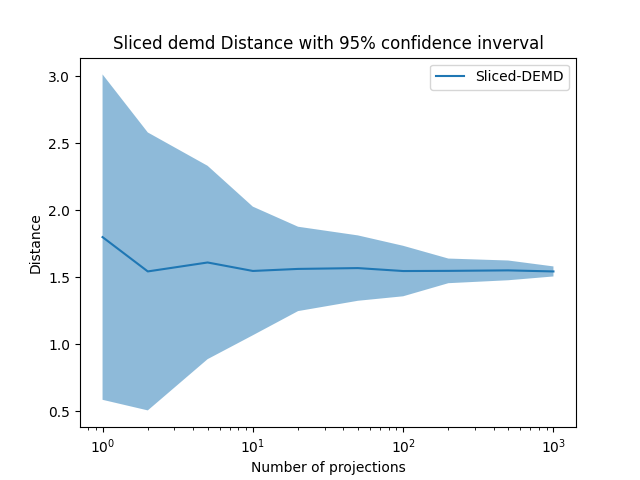
\includegraphics[width=0.32\textwidth]{figs/sliced/demd_mulidim_proj_convergence.png}
    % 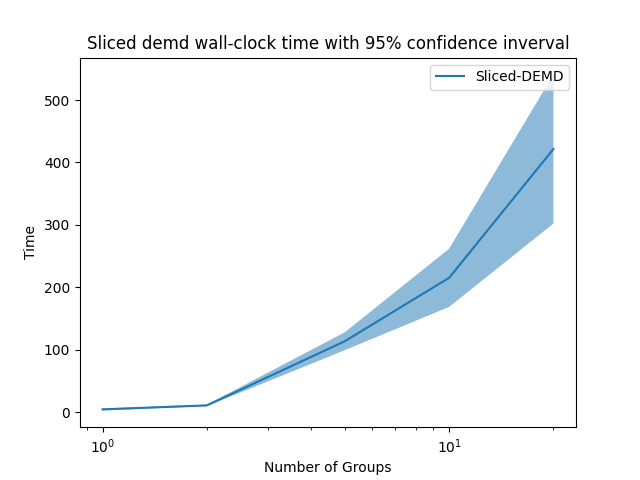
\includegraphics[width=0.32\textwidth]{figs/sliced/groups_vs_distance.png}
    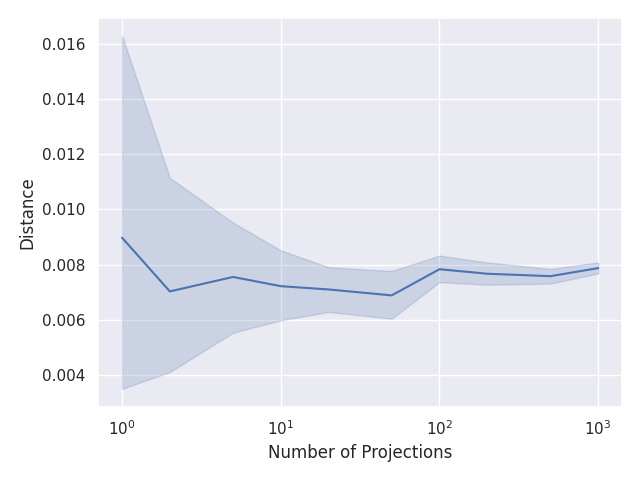
\includegraphics[width=0.4\textwidth]{6_demd/figs/sliced/demd_multidim_proj_convergence_CelebA.png}
    \caption{Sliced DEMD Distance as a function of number of projections.}
    \label{fig:sliced}
\end{figure}
%based on specific use cases.

One limitation of DEMD
is its inability to be directly applied to distributions over multi-dimensional discrete spaces, such as latent spaces common in generative models. 
% The nature of the cost and algorithm suggest this might be a nontrivial, but potentially interesting problem to study.
% In evaluating what might enable these extensions (over images, higher-order tensors, etc.), one important piece is generalizing the Monge cost in some reasonable form, given by an ordering over the multi-dimensional space. Importantly, \textit{a Euclidean embedding of our discrete space does not result in a Monge cost. \ronak{this is true for euc dist, but squared euc dist does satisfy monge}} A sufficient ordering could be defined by a space-filling curve in continuous settings (Hilbert/Peano curves may suffice), but this would not handle arbitrary dimensional spaces unless reduced to the 1-D setting as described above (and adds incremental utility for much more complexity). 
Slicing is a heuristic that has been shown to work well. To evaluate feasibility, we embed distributions over multi-dimensional continuous spaces, take random projections over 1-D spaces, and recompute our DEMD measure. Our gains in the many-distribution setting extend here as well: over a 64-dimensional latent space embedding of CelebA, we can efficiently compute our DEMD measure over all 40 attribute subgroups, and observe convergent behavior w.r.t. the number of projections.% (Fig.~\ref{fig:sliced}).
%Our scaling above enables distance computations in this setting as well, See Appendix~\ref{sec:app-multi} for additional details.

%{\bf Ethical Considerations.} Machine learning (ML) models that have skewed performance on subsets of individuals are increasingly of concern within the community. Our proposed DEMD can be used to address general fairness problems in ML, particularly where group disparities are to be mitigated. 
%We aim to add another tool in the fairness toolbox available to ML practitioners, alongside important cultural procedures promoting equitable use, from data sources to model outputs and human audits.

% While the goal of our tool is to mitigate group disparities in practice, it is not a catch-all solution to fairness problems in machine learning. Although the results presented are promising, any application of DEMD in practice should, as always, be done with care, including both algorithmic procedures such as full hyperparameter optimization and cross validation, as well as independent, human audits of all models and results.

% An intriguing direction for future work could exploit an unexplored feature of the generalized EM functional. In~\cite{kline2019properties}, it is shown that the optimal objective value of the generalized EM program is {\em Minkowski additive} in the program data. This is a highly unusual property. It may be possible to exploit this property to other use cases in machine learning models, as well as other theoretical investigations.


% \textbf{Minkowski Additivity}
% Means we can also separate and combine functionals on different sets, and optimizing one set until it is a subset of another allows us to take advantage of the additivity.

% \textbf{Fairness Intrinsic Dimensionality}
% The support outlined above is a measure of fairness dimensionality.
% A completely fair algorithm would have a dimensionality of 0.

